\documentclass{article}
\usepackage[utf8]{inputenc}
\usepackage{graphicx}
\usepackage[a4paper, total={170mm, 257mm}, left=25mm, top=20mm, right=25mm, bottom=20mm]{geometry}
\usepackage{hyperref}
\usepackage{float}
\usepackage{indentfirst}

\title{Report for Assignment 0, COL380}
\author{Shrey J. Patel, 2019CS10400}
\date{January 2022}

\begin{document}

    \maketitle 

    \tableofcontents

    \newpage

    \section{Analysis of Original Code:}
    The original code divides given data items into threads in a round robin fashion. This is implemented in the first pragma omp loop in the code of the file \textit{classify.cpp}.

    The rest of the code includes defining the rangecount array to store the number of accumulated data items before a given range. And then, the second loop divides the ranges in to threads in a round robin fashion. And for each range, the thread assigned to it iterates over all the possible data items to select those which fall in this range. Thus, the complexity of this sorting is O(r*d). \textit{(r = number of ranges, d = size of data)}.

    \subsection{Output}
    I have executed the given code for different number of threads, and the result is as expected i.e. higher the number of threads, lesser the average time of execution. 

    \begin{center}
        \begin{tabular}{|c|c|}
            \hline
            \textbf{$\#$threads} & \textbf{Avg. runtime} \\
            \hline
            4 & 437 ms \\
            \hline
            8 & 341 ms \\
            \hline
            16 & 311 ms \\
            \hline
        \end{tabular}
    \end{center}

    \subsection{gprof}
    The gprof output has no substantial information. It only shows the time taken by each function in the \textit{main.cpp} file. 
    
    \begin{figure}[H]
        \centering
        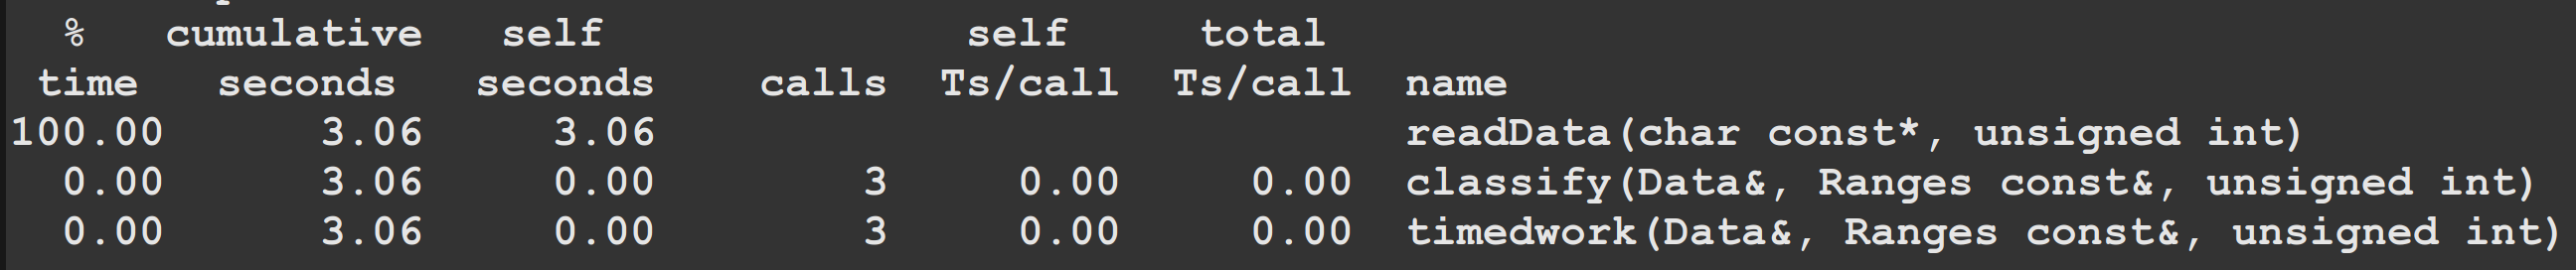
\includegraphics[width=15cm, height=2cm]{gprof_4.png}
        \caption{4 threads}
    \end{figure}
    
    \begin{figure}[H]
        \centering
        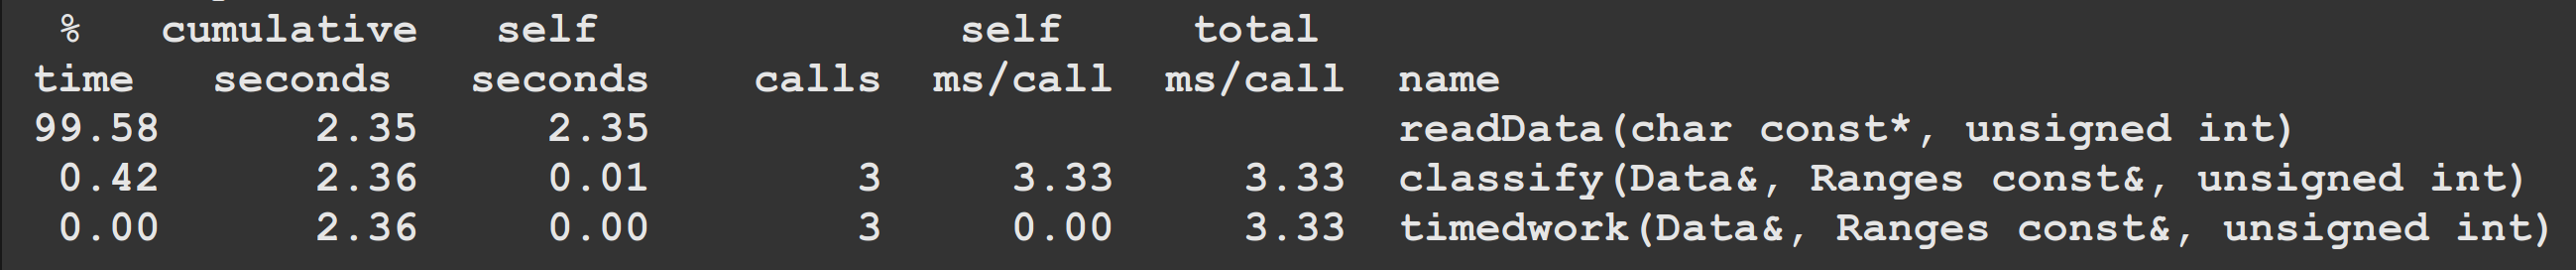
\includegraphics[width=15cm, height=2cm]{gprof_8.png}
        \caption{8 threads}
    \end{figure}
    
    \begin{figure}[H]
        \centering
        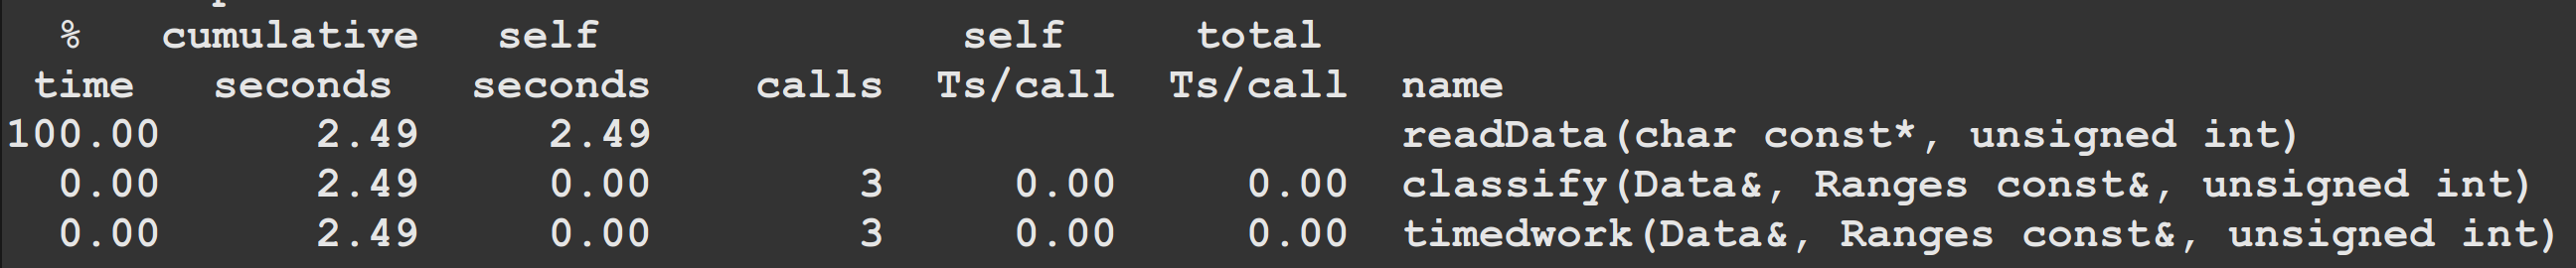
\includegraphics[width=15cm, height=2cm]{gprof_16.png}
        \caption{16 threads}
    \end{figure}
    
    Note that almost the entire time is elapsed in running the \textbf{readData} function because of the size of the input. And again, as the number of threads increase, the total time decreases.   

    \newpage
    \subsection{valgrind}
    Since all our changes are only in classify.h and classify.cpp, we will only consider the rows corresponding to these two files. Now, from the valgrind output files, almost all columns are same irrespective of the number of threads, except two columns in the row corresponding to classify.h
    
    \begin{center}
        \begin{tabular}{|c|c|c|}
            \hline
            \textbf{$\#$threads} & \textbf{D1mr} & \textbf{DLmr} \\
            \hline
            4 & 5008 & 37 \\
            \hline
            8 & 9432 & 118 \\
            \hline
            16 & 17940 & 278 \\
            \hline
        \end{tabular}
    \end{center}

    D1mr corresponds to read misses in L1 cache and DLmr corresponds to read misses in L2 cache. As the number of threads increase, the number of cache misses also increase, according to the table. This might be due to \textbf{false sharing} in local caches. This has been explained later in this report in detail. 
    
    \section{Analysis of Modified Code:}
    Since we know that \textit{gprof} doesn't provide any useful info regarding threading and caches, I have not provided any analysis of \textit{gprof} further in this report. But, the relevant output files are included in the submission.  Also, in the subsequent modifications, we assume the number of threads to be 4.

    \subsection{Optimization 1}
    In the first loop of the original code, the data items are divided into threads in a round robin fashion, which means that adjacent items will be allocated to different threads. Now, since adjacent data items have contiguous memory locations, and the local cache of a thread stores an entire cache line of contiguous memory addresses, each thread's cache will also inadvertently store adjacent items. Since the thread doesn't operate on these adjacent items, majority of the space in the cache line is wasted. 
    
    But if we can use these adjacent items, it would be highly efficient both in terms of cache space usage and in terms of cache rewrites (because earlier, the cache line needed to be replaced with another line so that the same thread can fetch another allocated data item, which was not adjacent). So, now instead of round robin fashion, we allocate adjacent items to each thread, in such a way that each thread gets roughly the same amount of data for better division of labour. 
    
    \subsubsection{Output}
    \noindent
    \textbf{Avg. runtime after optimization:} 540 ms \\
    
    At first, this might seem to be a worse strategy as evident from the increase in runtime with respect to the original code. But this has happened due to the nature of the given test case, in which the data is fairly sorted from the get-go. 
    
    Since, we are dividing the data items in an adjacent(block) fashion, the thread with greater tid value will be assigned larger data. So, while checking for the range(which is O(r) in the code), this later thread will possibly have data items which belong to the last range in the range array(Note that the ranges are given in sorted order in this case). So, the amount of disparity in computation is huge between initial threads and final threads. This results in unequal division of labour in such special cases. 
    
    The original code used round robin division, so fortunately, in this case, the larger data items were also divided equally among the threads, resulting in uniform distribution of computation. But, if the data and the ranges given in the testcases are shuffled, the optimized code would perform much better as explained above. So, the \textbf{optimized code is faster on average}.

    \subsubsection{valgrind}
    Comparing with the original code, the only difference seems to be in the classify.h row in the following columns:
    
    \begin{center}
        \begin{tabular}{|c|c|c|}
            \hline
             & \textbf{D1mr} & \textbf{DLmr} \\
            \hline
            original & 5008 & 37 \\
            \hline
            modified & 1604 & 27 \\
            \hline
        \end{tabular}
    \end{center}

    As evident from the table, this optimization results in lesser number of cache misses in both L1 and L2 caches. 

    \subsection{Optimization 2}
    As we discussed before, the complexity of the second loop is O(r*d), which can be improved to O(d), by first dividing the blocks of adjacent ranges into threads (as described in optimization 1), and then running an O(d) loop over each thread. 
    
    This requires changing the definition of rangecount array. Earlier rangecount[i] was defined as the number of data elements \textit{until} the range i. Now, rangecount[i] is defined as the number of data elements \textit{before} the range i, so the elements of range[i] will not be counted here. 
    
    \subsubsection{Output}
    \noindent
    \textbf{Avg. runtime after optimization:} 186 ms \\

    Such a decrease in runtime with respect to original code is expected because of the decrease in algorithmic complexity and better threading(using spatial locality).

    \subsubsection{valgrind}
    There is a huge contrast between the valgrind files of the original and the modified code after this optimisation. Some of the most important are listed below: 
    
    \begin{itemize}
        \item Because of the drastic change in the algorithmic complexity, there is a huge decrease in the number of instructions in both classify.cpp and classify.h
        
        \begin{center}
            \begin{tabular}{|c|c|c|}
                \hline
                \textbf{classify.h} & \textbf{Ir(classify.cpp)} & \textbf{Ir(classify.h)} \\
                \hline
                original & 6,067,562,072 & 4,031,538,840 \\
                \hline
                modified & 4,031,538,840 & 496,698,649 \\
                \hline
            \end{tabular}
        \end{center}
        
        \item There is a stark contrast in the number of cache misses as well. There a lot less read/write misses in the modified code. 
        
        \begin{center}
            \begin{tabular}{|c|c|c|}
                \hline
                \textbf{classify.cpp} & \textbf{D1mr} & \textbf{DLmr} \\
                \hline
                original & 126,266,194 & 1,005,469 \\
                \hline
                modified & 4,643 & 38 \\
                \hline
            \end{tabular}
        \end{center}
        
        \begin{center}
            \begin{tabular}{|c|c|c|}
                \hline
                \textbf{classify.cpp} & \textbf{D1mw} & \textbf{DLmw} \\
                \hline
                original & 127,017 & 126,811 \\
                \hline
                modified & 0 & 0 \\
                \hline
            \end{tabular}
        \end{center}
        
        \item But, in contrast, the number of write instructions in classify.h are much higher for the modified code as compared to the original code. 
        
        \begin{center}
            \begin{tabular}{|c|c|}
                \hline
                \textbf{classify.h} & \textbf{Dw} \\
                \hline
                original & 1,009,072 \\
                \hline
                modified & 51,879,635 \\
                \hline
            \end{tabular}
        \end{center}
        The main reason of this is the extra writes on the rangecount array that we are doing in the modified algorithm. In the original code, we were using a single local variable for each thread. Additionally, the rangecount array is shared, which further contributes to the number of writes since its consistency has to be maintained at each cache level.  
        
    \end{itemize}

    \subsection{Optimization 3}
    Previously in optimization 2, we used rangecount to sort the data items into given ranges. But rangecount array is shared between all the threads. Although there are no race conditions since the ranges are uniformly distributed among the threads, there is still a chance of false sharing due to cache invalidation. This can be avoided if we copy the contents of the rangecount array into a local count array for each thread.
    
    This decreases the number of extra write-backs and cache misses caused due to false sharing. 
    
    \subsubsection{Output:}
    \textbf{Avg. runtime after optimization:} 173 ms

    This runtime is similar to the case of optimization 2, since only few

    \subsubsection{valgrind}
    From observations, there is \textbf{no perceptible difference} in the valgrind outputs of optimization 2 and optimization 3. Theoretically, the optimisation 3 should lead to lesser number of read/write misses as well as lesser number of write instructions since we are using a local count array instead of a shared count array.

    \subsection{Other possible optimizations}
    \begin{enumerate}
        \item 
        \begin{itemize}
            \item In above optimizations, we have divided the task into threads with respect to the number of ranges i.e. we try to divide so that each thread gets equal number of ranges. But the actual computation is in on the data items rather than the ranges. For example, a given testcase may contain all data items concentrated in the ranges assigned to a single thread as opposed to being scattered across all the given ranges. If we continue using the older strategy, then all the computation will be concentrated in the same thread, while all the other threads will remain idle for most of the time. This is not an efficient divison of labour. 
            
            \item So, instead of dividing the ranges on the basis of their indices, we can divide them on the basis of their data items. So, each thread will have about the same number of data items assigned to it. To implement this, we assign the starting and ending indices of the ranges to each thread, so that the sum of data items assigned to each thread is as uniform as possible(using close to average number of data items in each thread).
            
            \item I have not not included this optimization in the modified code since it doesn't result in the decrease of runtime, because of the large pre-computation overhead. 
        \end{itemize}   
        
        \item 
        \begin{itemize}
            \item 
            In the code, the Counter array counts[] stores the counter of each range. And each Counter object stores the count accumulated by all threads, which is then stored in the internal array $\_$counts. This means that each thread is responsible for writing on its cell in this array, for each counter. 
            
            \item But because caches work in cache lines and since the array elements are stored in contiguous memory addresses, a collection of adjacent cells are stored in the local cache of a thread, depending on the size of the cache line. 
            
            \item So, the local cache of a thread may contain a location which the thread will never write upon. But because of false sharing, if some other thread mapped to that memory location writes in that cell in its own local cache, then the entire cache line will be invalidated along with the current thread's cell. So, the whole cache line will be written through lower caches, before the current thread can retrieve its corresponding cell again. Thus, false sharing may cause extra write backs and therefore more time.
    
            \item One way to address this is to increase the alignment of the elements in the $\_$counts array so that each cell is aligned to the cache line size. This will decrease the number of non-relevant memory locations in the cache with respect to the current thread and thus decreasing the chances of false sharing.
    
            \item Maybe, this alignment could have been changed using alignas() in the Counter class. I have not implemented this optimization since I am not clear how alignas() works, and I am also not aware of the size of a cache line.
        \end{itemize}
    \end{enumerate}
\end{document}